% git-ui-thesis.tex
% Created: 3/4 2015

%\documentclass[12pt,a4paper,article,compsoc]{IEEEtran}
%\hyphenation{op-tical net-works semi-conduc-tor}
\documentclass[a4paper,oneside]{bth} % I WANT "twocolumn"!!!
\usepackage{paralist}
\usepackage{cite}
\usepackage{hyperref}
\usepackage{float}
\usepackage{tabu, tabularx, caption, subcaption}
%\usepackage{graphicx}

\usepackage{amsmath}
\usepackage{mathenv}
\usepackage{amssymb}
\usepackage{amsthm}
\usepackage{textcomp}
\usepackage{longtable}
\usepackage{multirow}
\usepackage{pifont}
\usepackage{changepage}
\usepackage{listings}
\usepackage{url}
\usepackage{xspace}
\usepackage{xtab}
\usepackage[utf8]{inputenc}
\usepackage[T1]{fontenc}
\usepackage{graphicx}
\DeclareGraphicsExtensions{.pdf}

\begin{document}
		\pagestyle{plain}
		\pagenumbering{roman}
		
		% Front matter
		{\pagestyle{empty}
		\changepage{5cm}{1cm}{-0.5cm}{-0.5cm}{}{-2cm}{}{}{}
		\noindent%   
			{\small
				\begin{tabular}{p{0.75\textwidth} p{0.25\textwidth}}
					\textit{Bachelor Thesis}&\multirow{4}{*}{\bthcsnotextlogo{3cm}}
					\\
					\textit{Computer Science}
					\\
					%\textit{Thesis no: MCS-2015-NN}
					\\
					\textit{08 2015}
					\\
				\end{tabular}
			}
			\begin{center}
				\par\vspace {7cm}
				{\Huge\textbf{Git - CLI or GUI}}   
				\par\vspace {0.5cm}
				{\Large\textbf{Which is most widely used and why?}}                   
				\par\vspace {3cm}
				{\Large\textbf{Robin Olofsson}}
				\\
				{\Large\textbf{Sebastian Hultstrand}}
				\par\vspace {7cm}
			\end{center}

			\noindent%
			{\small Department of Software Engineering 
			\\
			Blekinge Institute of Technology
			\\
			SE--371 79 Karlskrona, Sweden}
			\clearpage
		}

		{\pagestyle{empty}
			\changepage{5cm}{1cm}{-0.5cm}{-0.5cm}{}{-2cm}{}{}{}
			\noindent%
			\begin{tabular}{p{\textwidth}}
				{\small This thesis is submitted to the Department of Computer Science \& Engineering at Blekinge Institute of Technology in partial fulfilment of the requirements for the degree of Bachelors of Science in Computer Science. The thesis is equivalent to 20 weeks of part-time studies.}
			\end{tabular}
			\par\vspace {12cm}
			\noindent%
			\begin{tabular}{p{0.5\textwidth}lcl}
				\textbf{Contact Information:}\\
				Author(s):
				\\
				Robin Olofsson
				\\
				E-mail: Olofsson\_@live.se
				\\
				Sebastian Hultstrand
				\\
				E-mail: Sebastian@storm-net.se
				\\
				\par\vspace {5cm}
				University advisor:
				\\
				Assistant Prof.\ Conny Johansson
				\\
				Department of Software Engineering 
				\par\vspace {1cm}
				\noindent%
 				\\
				Department of Software Engineering  & Internet & : & www.bth.se/didd\\
				Blekinge Institute of Technology & Phone	& : & +46 455 38 50 00 \\
				SE--371 79 Karlskrona, Sweden & Fax & : & +46 455 38 50 57 \\
			\end{tabular}
			\clearpage
		} % Back to \pagestyle{plain}

		\setcounter{page}{1}

		% ABSTRACT
		\abstract
		\begin{changemargin}{+1cm}{+1cm}
			\noindent
				A lot of us have encountered the discussion about which one of the command-line interface or the graphical user interface is the better one in terms of interfacing with Git.
				This thesis is an attempt to find out which user interface new Git users prefer for Git and what experienced Git users prefer.\\
				We aimed to find out if there's anything significant which can be gained from using either of the interfaces in comparison to each other. Lastly we tried to answer the question "At what stage of Git proficiency would you stand to gain the most from the command-line interface or the graphical user interface?".\\
				We have collected data through three interviews and a survey, which yielded approximately 370 responses.\\
				Based on our results we've found that the command-line interface is the more popular user interface, in general, amongst Git users.
				\\We've also found that most users back out of using graphical user interfaces, as their primary user interface, as they get more experience with Git. They usually change their primary user interface to a command-line interface or continue to use both the graphical user interface and the command-line interface together.
				The results from our study regarding why, is presented in this thesis.
				

			\par\vspace {1cm}
			% 3-4 keywords, maximum 2 of these from the title, starts 1 line below the
			% abstract.
			\noindent
			\textbf{Keywords:} Git, Interfaces, VCS, New users, Experienced users
		\end{changemargin}

		\tableofcontents 
		\listoffigures %in case you have them
		%\listoftables %in case you have them
		%\listofalgorithms %in case you have them
		
		\cleardoublepage
		\pagestyle{headings}
		\pagenumbering{arabic}
		
		% Settings of author and title
		\title{This title is not determined yet}
		\author{Robin~Olofsson and Sebastian~Hultstrand}
		
		% Content
		\chapter{Introduction}
		Git is a very popular version control system out there today, along with version control systems like SVN and Mercurial. The discussions between using CLIs' (Command-line interfaces) or GUIs' (Graphical user interfaces), in general, have been going on since the late 70's and early 80's when operating systems like the Lisa and Macintosh among others came out \cite{HistoryOfGUIWiki} and the GUI revolution was kicked into high gear.
		To date people seem to prefer the CLI over GUI when working with Git based on own experiences and the results from the GitSurvey in 2012\cite{GitUserSurvey}, however it is not clear as to why.
		Theories do exist which state that the CLI provides a faster and more controlled way of dealing with Git. \cite{GitUserSurvey}\cite{GitInClassroom}
		\\
		The reason this topic was thought of in the first place was due to an observation made in one of our courses. As of the day of writing there is no real formal introduction course to version control at Blekinge Institute of Technology, much less to Git. Instead there are a small number of courses where students are introduced to Git alongside the actual content of the course and most of the learning is left to what the student chooses to find out.\\
		During one of these introductory talks about Git the students were encouraged to start out by using the command-line interface in order to get a feel for how Git works. This was met by a lot of complaining from the students as they would rather use a graphical user interface. The subsequent discussion that ensued was the spark that lit the idea to do this research.
		\\
		In this paper we've taken a closer look into what people use today, in terms of interfaces to work with Git, and if there's any correlation to be found between how people use Git and which interface they used.
		The aim was to find out which interface is more preferred, which is more suitable to novice users and if developers can benefit more from using either of the two interfaces when reaching a certain knowledge-level of Git. Novice Git users and developers are therefore the target audience for this paper.\\
		To find these answers we have conducted a survey, through an online service (Google forms), that was sent out to developers within the industry of software manufacturing and students at Blekinge Institute of Technology. The distribution to the industry was done through in part people we know whom agreed to spread the link to co-workers and so on, and in part through online forums. \\
		A literature study has been carried out as well, mainly to help  gather as much knowledge about current opinions within the scientific scene about the CLI and GUI interfaces.
		Thanks to the clues found in the literature review we could develop questions that would provide us with relevant data.\\
		Three interviews were conducted to get a deeper understanding of the answers that were gathered through the survey.
		We felt that a survey could possibly provide enough information to carry out the work but by conducting interviews there was a greater chance of understanding as to why the participants, of the survey, answered the way that they did.
		
		% Background
		\chapter{Background}
			\section{Git}
			In 2005 the Linux development community started the development of Git.
			Up until that point they had been using BitKeeper as their version control system. By that time BitKeeper was free but when the company behind the product decided to price it the Linux development community quickly abandoned the solution to develop their own open-source version control system.\cite{ProGit}
			To date, Github alone has over 21.7 million repositories.\cite{GithubAbout} All of these repositories are different little packages of code or text that people have created and are working on, with varying levels of frequency.
			Git is, today, one of the most common version control systems \cite{EclipseDeveoperReport}\cite{DeveloperProductivity}\cite{MicrosoftSurveyResults}. The reason for Git being a very powerful tool is its flexibility in work flow choice, the storage is well designed and consistent,\cite{WhyGit} and the surrounding functionality is adaptive and highly customizable. This contributes to two things, the learning curve being quite steep and a challenge to get over. But once you get over the curve you can very easily oversee and understand the functionality and structure of a Git repository and have little difficulty learning new methods and work flows. This at least seems to be the consensus on forums and message boards around the web, and it coincides quite accurately with our experiences as well.
			\\
			The basic structure of a Git repository is; 1) a .git directory that houses the meta date and object database for your repository and all the committed changes. 2) A staging area where changes that are to be committed are kept in waiting for a commit to take place. 3) A working directory where your plain working copy of the source code is held. This is where development is done. \cite{GitStructure} 
			So depending on what version of the code you checkout from the .git directory, it will appear in the working directory. Then you code your changes and stage them, thus placing the changes securely in the staging area. The final step is to commit what is in the staging area and it will be saved into the .git directory. Some repositories have a remote host that the changes can be pushed to for ease of sharing the code. These are the very basics of how Git works \cite{GitStructure}
			
			\section{Command-line interface and the Graphical user interface}
			There are two main ways of interfacing with Git, one is through a command-line interface and the other is through one of many graphical user interfaces that are available. \cite{GitGUIs}\\
			
			When using the command-line interface you type commands manually to preform the desired actions whilst in a graphical user interface you will have something visual to interact with, such as buttons, input fields and so on.
			There are pros and cons with using either of the two interfaces not only for Git but in general.
			For example, through a command-line you can rename 100 files with a lot less effort than with a graphical user interface. Though it would require you to know the commands needed to rename the files. One command can perform a lot of different tasks, whilst in a graphical user interface you would normally have to rename each file one by one which would require a lot more time but less knowledge. As mentioned in the introduction the debate of GUI v. CLI has been going on since the 80's and not a great deal has changed in the arguments, since they are so deeply ingrained in either interface. 
			A good analogy is the car dealership comparison made in the article (Later a book) \textit{In the beginning was the command-line} (Stephens, 1999) \cite{InTheBeginning}. The summary of the analogy would be that there are a bunch of competing automotive dealerships on the same street where some are expensive, but easy to use and fairly cheap to repair however they often break down. Another sells sleek euro-style cars that no one really knows the inner workings of, they are expensive but beautiful. Then there is the super advanced tanks that are being given away for free. Yet still all the customers go for the cheap car that is sort of bad or the expensive euro-car. No one wants a tank even though they are free, because no one can be bothered to learn how to drive it. 
			This analogy helps to illustrate the situation between the GUI and CLI very simply but quite accurately.
			\\\\
			"A command line interface (CLI) enables users to type commands in a terminal or console window to interact with an operating system. Users respond to a visual prompt by typing a command on a specified line, and receive a response back from the system. Users type a command or series of commands for each task they want to perform."\cite{OracleCLIAndGUI}.\\
			An example of such an interface for Git can be seen in Figure 2.1 below.
			
			\begin{figure}[H]
				\centering
				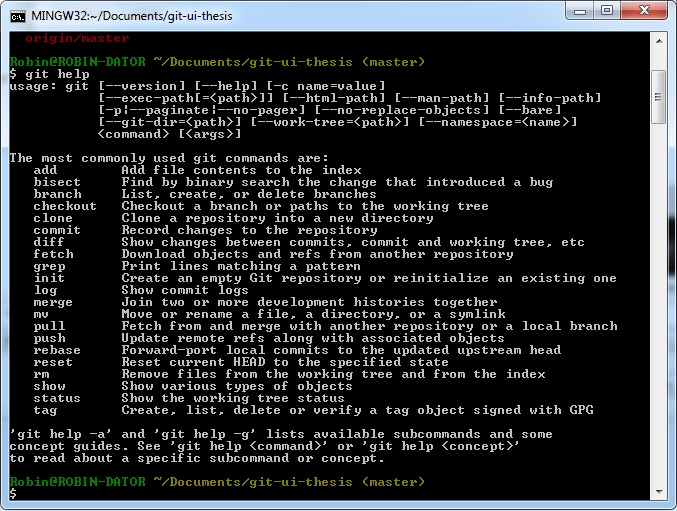
\includegraphics[width=0.8\linewidth]{git-cli.jpg}
				\caption{Git command-line interface, in Windows}
				\label{fig:git-cli}
			\end{figure}
			
			Whilst - "A graphical user interface (GUI) uses graphics, along with a keyboard and a mouse, to provide an easy-to-use interface to a program. A GUI provides windows, pull-down menus, buttons, scrollbars, iconic images, wizards, other icons, and the mouse to enable users to interact with the operating system or application." \cite{OracleCLIAndGUI}.\\
			An example of such an interface for Git can be seen in figure 2.2 below.
			
			\begin{figure}[H]
				\centering
				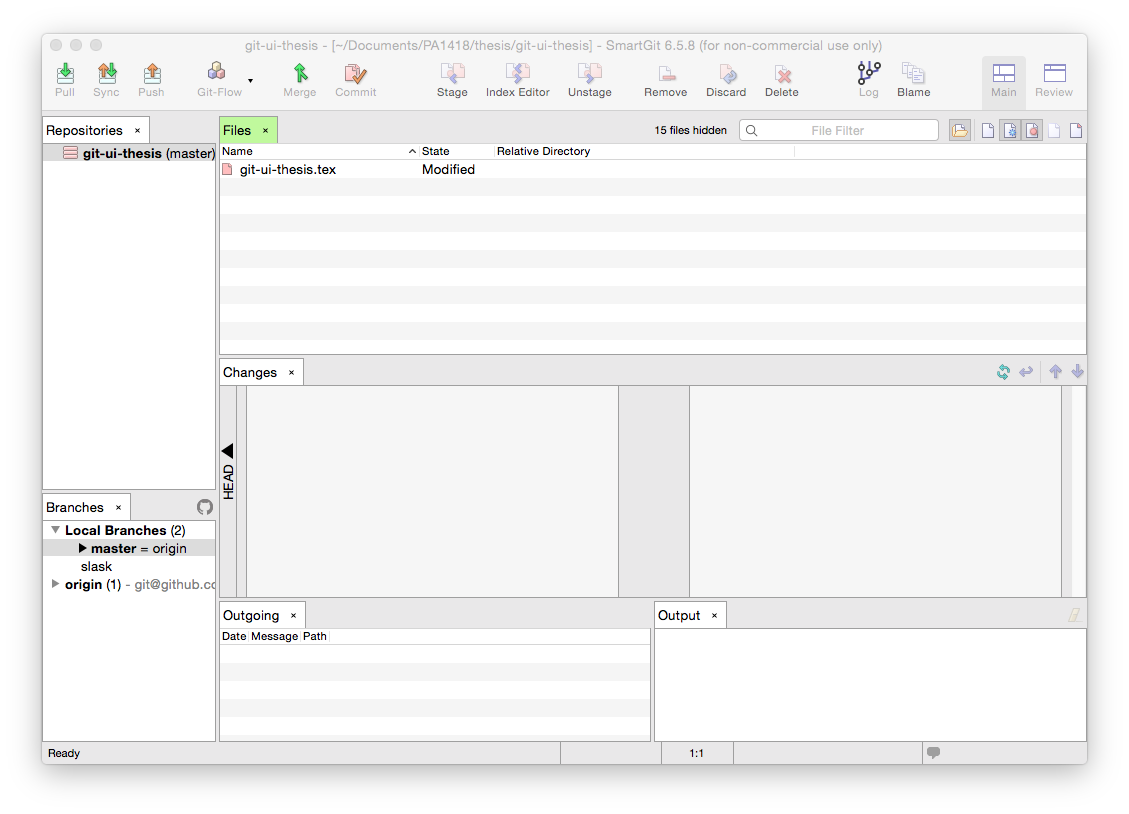
\includegraphics[width=0.8\linewidth]{git-gui.png}
				\caption{Git graphical user interface, Smart Git Hg on OSX}
				\label{fig:git-gui}
			\end{figure}
			
			\section{Terminology used}
			\begin{itemize}
				\item Demographic - The word demographic is used in this thesis and refers to a certain group that answered our survey. The group's members are defined by their indicated level of proficiency with Git, and the amount of experience they have with Git. The determination of which demographic a respondent falls in is made up of a point system. The alternatives are given an arbitrary point value to signify rank and when the points for the chosen alternatives are added up we get the sum for the respondent. Low is defined as 2-4, mid 5-7 and high 8-9. We did this in order to make it possible to split the respondents into demographics.
				\item VCS - A VCS is a system that records changes to a file or a set of files over time so that you can recall specific versions later.
				There are three different types of version control systems; Local Version Control Systems, Centralized Version Control Systems and Distributed Version Control Systems.\\
				Since Git is a Distributed Version Control System and this thesis concerns Git - you can safely assume that we discuss about the Distributed Version Control System when we say Version Control System.\cite{typesOfVCS}\\
				Version control systems usually consists of two applications, one on a server-side and one on a client-side.
				The basic functionality of a VCS is to maintain source code, other types of software files and their history.\cite{FoundationVCforWebDevs}
				
				Initially, you either create a new project or import a project into the VCS.
				Once that's done you check out a version of the project into your private working directory and after that it's time to get to work and start coding.
				Every time you feel like you are content with a change you've made, such as a bug fix or the addition of a new feature, you commit your changes to the repository alongside with a explanatory message to let everyone know what's new/changed.
				Then, every once in a while, you update/synchronize your private version of the project with the changes your colleagues have committed.
				This action will allow all of your colleagues to have roughly the same source code base. From there on out you and your colleagues can battle against the mistakes that has been produced  and once you feel confident enough on the software you can roll out a release.\cite{vcsExplanation}
				\item UI - The word is an abbreviation of the term user interface and refers to either a graphical user interface, the command-line interface or both.
				\item CLI - Command-line interface.
				\item GUI - Graphical user interface.
			\end{itemize}
			
		% Research methodology
		\chapter{Research methodology}
			\section{Research questions}
			\begin{enumerate}
				\item What is most commonly used when getting started with Git, CLI or GUI?
				\item What is most commonly used by experienced Git users, CLI or GUI?
				\item What can be gained from using the GUI in comparison to the CLI, in the aspects of functionality and convenience?
				\item What can be gained from using the CLI in comparison to the GUI, in the aspects of functionality and convenience?
				\item At what stage of Git proficiency would you stand to gain the most from the CLI or the GUI? (Looking at what should you start out with to learn how Git works and how it is used, and what you will gain the most from when you get to a higher level of understanding Git.)
			\end{enumerate}
				\subsection{Reasoning for questions}
				We initially identified and used the above questions as the basis for our work because they work well as guidelines towards what we wanted to find out. Firstly we had to find out which UI new Git users use and how they got started with Git, in order to see what the reality is today. Secondly we had to look at what more experienced users employ currently in terms of UIs, in order to see how the trend of swapping appear to be. This is something we could do through looking at the results from our survey and the Git survey from 2012 \cite{GitUserSurvey}. Thirdly we wanted to examine a few examples of the UIs available in order to see what could be gained, in terms of functionality and convenience. But since we lacked time and the knowledge, we couldn't do a clear objective analysis of the UIs. Instead we used some of the opinions and reflections about the UIs gained from the survey and the interviews to get an idea of what users have gain through using the UIs. 
				Fourthly we wanted to examine all the results collected while researching the other questions in order to build at least a partial answer to the fifth question.\\
				The reason that we thought this would be important is that there are so many different approaches to learning git and so many opinions that you have to get through before you can decide how you want to learn. These results may help shortening that period.
			\section{Approach for answering research questions}
			To answer the research questions a literature study was conducted to find out how Git works, workflows and discussions about the command-line interface and about graphical user interface in general. Based on what was found, the design of the survey and a number of questions for the interviews was created.\\
			The intention of the survey was to collect information about current users preferences and perceptions. We wanted to know what they were currently using (either CLI or GUI tool), how long they have been using it, what their perception of the two different types of interface were, how they work with Git, how they began using it and how they learnt to use it. 
			Using this information we attempted to idenfity correlations between their experience with Git, how they use Git and their preferences and reasoning behind their choice of UI.\\
			The interviews were based on more open questions where the aim was to allow the subject to elaborate around why they have chosen to work like they do, and discuss the perks of the two different types of interfaces that we put forward. The aim of the exercise was to get a deeper understanding of the reasoning that goes into their choices which is an understanding that the survey would not be able to supply.\\
			Studies have been conducted to try to find out what people use when interfacing with Git, but the most recent study to cover that area, that we could find was conducted in 2012 \cite{GitUserSurvey}.
			By conducting a survey, where we aimed to find out what people use today and why, there was the possibility to gather fresh data as the data collected back in 2012 might not accurately represent how people interface with Git today.
			\\\\
			In summary questions 1 and 2 was answered using the survey where questions pertaining to what UI the subject was currently using and what UI the subject began using for Git interfacing. Correlations was searched for in the 2012 GitSurvey \cite{GitUserSurvey} to see how the results compare to other studies.
			Questions 3 and 4 was answered in part through some of the perception related questions in the survey coupled with the interviews. Finally question 5 was somewhat answered by, in part, statistics from the survey by looking at questions pertaining to perception of the UIs, time consumption associated with the subjects use of Git. Both general and problem based, and the subjects varying use of and proficiency with Git. Also partly through the interviews where we were able to hear what drew the subjects to the UI that they use and what they believe to be important in the choice of a UI. Since we were able to determine the demographics based on the level of proficiency, from the survey we could use those to find and interview subjects which represented a certain demographic and discuss their needs and requirements from the user interfaces. 
			Our belief was that, by answering questions one to five, developers would get a general overview about how present days Git users interface with Git and why. The "why" didn't have to be detailed for the information to be valuable because it might be enough to know that, hypothetically, making a commit and pushing code through a graphical user interface is slower than doing the same in the command-line interface.  
		 
			\section{Literature review design}
			In our literature study we used BTH Summon, Engineering Village, IEEE Xplore and Google scholar as our primary search database.\\\\
			\textbf{Keywords used:} Git, configuration control, version control, public domain software, software engineering, linux, UI, User interface, Graphical user interface, GUI, CLI, Command line interface, Case study, User experience, Usability, UX, Interface.
			\\\\
			Our goal was to find literature where the authors examined the CLI, a GUI, or performed experiments with either or both the UIs. Papers that include this type of content is considered, by us, relevant to us.
			The age of the content did not matter to us, because we were interested in finding out how people's views of the CLI and GUI have changed throughout the years.
			To sort out what literature that was relevant we read the abstracts.
			Whenever we found a literature that had a relevant abstract we would then proceed to add it to a stack with literature that we believed to be relevant to our work.
			We initially performed one round of snowballing, through that round we found roughly 10 papers that we believed to be relevant. We did attempt a second round of snowballing, but unfortunately we didn't find any new and relevant literature, so we decided to conclude our search for literature by then.
			
			
			\section{Empirical study design}
			
				\subsection{Survey}
					\subsubsection*{Goal with the survey}
					The survey consisted of 13 multiple choice questions, the questions were aimed to be as easy and quick to answer as possible in order to persuade people to answer the survey. The survey was aimed at finding out the following: 
					
					\begin{itemize}
						\item Find out what level of experience the subject has with Git.
						\item Find out what UI they are currently using.
						\item Find out how the subject learnt Git.
						\item Find out what the subject gprimarly use Git for.
						\item Find out what operating system the subject has.
						\item Find out how much time the subject spend on average interacting with Git.
						\item Find out how often the subject need to consult another person, resource online or handbook to solve a issue related to Git.
						\item Find out how the subject precieves the GUI and the CLI, by word association. 
					\end{itemize}
					The questions we chose to include are the bare minimum we needed to try to achieve our goal with the survey. We tried to design them in a simplistic manner that should generate data concerning how the participants worked with Git. Just finding out how the respondents work with Git makes a huge impact as a interface might be more suitable for a certain types tasks due to it's set of functionality and the way it operates.
					Experience was another factor we wanted to include as it could possibly influence the choice of interface.
					
					\subsubsection*{Questions and alternatives}
					\begin{enumerate}
						\item How long have you been working with Git?\\
						\begin{inparaenum}[\itshape a\upshape)]
							\item \textless 6 months
							\item 6 months - 1 year
							\item 1-3 years
							\item 3-5 years
							\item 5-10 years
						\end{inparaenum}
						\item How would you rate your knowledge of Git?\\
						\begin{inparaenum}[\itshape a\upshape)]
							\item Novice
							\item Average
							\item Professional
							\item Master
						\end{inparaenum}
						\item What type of user interface are you primarily using for Git?\\
						\begin{inparaenum}[\itshape a\upshape)]
							\item Command-line interface
							\item Graphical user interface
							\item Both equally
						\end{inparaenum}
						\item How did you learn to use Git?\\
						\begin{inparaenum}[\itshape a\upshape)]
							\item Colleague or friend
							\item Open source community
							\item Online tutorials
							\item Book
							\item Course
							\item Self taught
						\end{inparaenum}
						\item What interface did you use when starting out with Git?\\
						\begin{inparaenum}[\itshape a\upshape)]
							\item Command-line interface
							\item Graphical user interface
						\end{inparaenum}
						\item Why do you use the interface you use today?\\
						\begin{inparaenum}[\itshape a\upshape)]
							\item Personal preference
							\item Standards for work environment
							\item Outside influences
							\item It is what i know best
						\end{inparaenum}
						\item What operating system do you primarily use?\\
						\begin{inparaenum}[\itshape a\upshape)]
							\item Windows
							\item Mac
							\item Linux
						\end{inparaenum}
						\item What do you mainly use Git for?\\
						\begin{inparaenum}[\itshape a\upshape)]
							\item Basic change tracking
							\item Collaborative work
							\item Large scale version control with branch management and code reviewing through Git
						\end{inparaenum}
						\item How many minutes per hour of development time, on average, do you spend on interfacing with Git?\\
						\begin{inparaenum}[\itshape a\upshape)]
							\item \textless 5 min
							\item 5-10 min
							\item 10-15 min
							\item 15-20 min
							\item 20-25 min
							\item 25-30 min
							\item \textgreater 30 min
						\end{inparaenum}
						\item How many times during a work day do you need to seek help for an issue with Git?\\
						\begin{inparaenum}[\itshape a\upshape)]
							\item 0
							\item 1-2
							\item 2-4
							\item 4-6
							\item 6-10
							\item 10-15
							\item 15-20
							\item \textgreater 20
						\end{inparaenum}
						\item What words do you associate with a Git GUI (Graphical user interface)?\\
						\begin{inparaenum}[\itshape a\upshape)]
							\item Aesthetic
							\item Easy
							\item Bulgy
							\item Auto-magic
							\item Difficult
							\item Helpful
							\item Simple
							\item Intuitive
							\item Insightful
							\item Hard
							\item Time consuming
							\item Cool
							\item Professional looking
							\item Control
							\item Difficult
							\item Ugly
							\item Old fashioned
						\end{inparaenum}
						\item What words do you associate with the Git CLI (Command-line interface)?\\
						\begin{inparaenum}[\itshape a\upshape)]
							\item Aesthetic
							\item Easy
							\item Bulgy
							\item Auto-magic
							\item Difficult
							\item Helpful
							\item Simple
							\item Intuitive
							\item Insightful
							\item Hard
							\item Time consuming
							\item Cool
							\item Professional looking
							\item Control
							\item Difficult
							\item Ugly
							\item Old fashioned
						\end{inparaenum}
						\item Which type of Git interface would you recommend others to use, no matter skill level?\\
						\begin{inparaenum}[\itshape a\upshape)]
							\item Command-line interface
							\item Graphical user interface
							\item Both
						\end{inparaenum}
					\end{enumerate}
				
					\subsubsection*{Crafting and distribution}
					The survey was made as a web form that we can easily collect the data from and most of all distribute easily. Distribution of the survey was done through a number of different channels such as BTH:s student mail list, friends working with software development in Sweden whom spread the survey as well and finally 8 different sub-reddits (Forum boards at the popular web forum Reddit) associated with software development (Look in the acknowledgements for the exact names of the sub-reddits). These gave a very large portion of the replies to the survey as a few of the sub-reddits that we managed to find were specifically for Git users. This generated some very fortunate feedback and interest from that community.
					To get as many responses as possible the survey was designed to be easy and quick to fill out and to motivate participants even further we had a prize drawn amongst the participants for three, one month gift subscriptions to the curio service Loot Crate. \cite{lootcrate} 
				
					\subsubsection*{Analysis of survey}
					The survey was crafted so that it can be evaluated and analysed in conjunction with the interviews. 
					First a demographic for the replying party will be determined based on their answers to questions one and two. This demographic was used when looking at the questions about what user interface they use and have used, their reasoning for using it and their perceptions of the user interfaces. The demographic was necessary to determine since the fifth research question is based on both experienced and inexperienced users.\\
					We made cross tabulations between what OS the respondents use/how they learnt Git/what they mainly use Git for and what interface they are using now. A conscious decision was made to make correlation analyzes between experience with Git and what interface the respondents use. This is something we had to do because the cross tabulations alone wasn't enough.\\
					The cross tabulations and the correlation analyzes can be found in Appendix B.
					\\
					Questions three and five, in the survey (check Appendix A Figure A.2a and A.3a), was used to determine the answer to the first research question and in conjunction with the determined demographic to answer the second research question.
					\\
					The rest of the questions on the survey (Questions 4, 6 - 13) was used as factors for answering the third, fourth and fifth research questions. As they pertain to difficulties, perceptions and opinions about the user interfaces. When coupled with the results from the interviews and the study of the user interfaces mentioned in section 3.2. They would place weight on elements that are found, thus allowing the determination of what parts of a user interface to Git, that the different demographics value or are influenced by. Graphs was crafted in order to easily convey the messages that the collected data holds. For example bubble graphs to look at how the different demographics are responding to the word association questions to find relationships between ability and perception of the interface type. 
					\\
					The data that was collected through the survey was stored in a Google spreadsheet \cite{GoogleSpreadsheet} and through that spreadsheet we parsed the resulting XML (Extensible Markup Language) into a MySQL database where querying the data to build datasets for graphs is a lot easier.
					Through the diagrams we could easily find out percentages of how many answered a question in a certain way and through that we could draw conclusions to help us in answering the research questions.
					
				
				\subsection{Interviews}
				The interviews were conducted with a small group of subjects that were representative of the different demographics that answered the survey. The way that we determined a demographic in this context was the level of proficiency with Git that the subject indicates they had and how long the subject had been using Git for. 
				These two aspects allowed analysis on a deeper level, of the needs and wants of different user groups. The minimum demographics to cover are new users of Git whom was learning to use Git at the moment and experienced users whom had been using Git often and for a longer time. The identifiers for these two groups are;
				\begin{itemize}
					\item[Group 1 - New users.]
					These users have less than one year of experience and identify themselves as Novice or Amateur users.
					\item[Group 2 - Experienced users.]
					These users have more than two years of experience and identify themselves as Pro or Master users.
				\end{itemize}
				There are no clear guidelines that we've followed in the creation of these groups, it was based on common logic by us. It seemed like a logical approach to assume that a user either has experience with Git or a user doesn't, which is how we categorized them into Group 1 and 2.
				
					\subsubsection*{Interview format}
					The format of the interviews was a discussion on the topic of this paper where the aim was to get the subjects to explain their standing on the issue of CLI v. GUI in Git interaction, and most of all elaborate around perceptions and experiences that they have. We did supply some information about the UI:s to allow the sessions to go into as much detail as possible. 
					We conducted three interviews with subjects from both of the above mentioned groups and one with a user with an indicated level of knowledge to be in between the two groups. The sessions were recorded and transcribed later to minimize the loss of information that would occur if we only took notes during the interviews.\\
					At the end we carried out a small quality analysis of the results.
					
					\subsubsection*{Questions and topics to discuss}
						\begin{itemize}
							\item What functionalities do you most often use?
							\item How do you perceive working with a Git GUI?
							\item How do you perceive working with Git CLI?
							\item Which, if any functionality do you miss in the interface you use today? In terms of ease of use, efficiency and comfort.
						\end{itemize}
						
						These questions were aimed at finding out more about what the subject needs and wants from the interface he or she works with. However the factors that needed to be taken into account when looking at this are how much the subjects knows about the interfaces, what type of work they actually do in Git and if the work is collaborative or not. These factors were covered in either the responses to the survey or the interview itself and was taken into account in the discussion.
				%\subsection{User interface analysis}
				%The analysis will not be conducted according to any usability metrics or heuristics scale. The analysis will consist of looking at what is possible to do in either of the interfaces, functionality and ability to customize behaviour in order to optimize the way you work with the interface. Since the interfaces are very different and we do not possess the knowledge and tools needed we will not take aesthetics into account. Since graphical user interfaces and the command-line interface have a basic set of functionality that are going to perform roughly the same tasks we will not take the basic functions into account, like staging, committing, merging, pushing, pulling, cloning and so on.
				%The analysis will be a simple high level overview of the haves and don't-haves of the interfaces, basically a pros and cons list, this in order to stay objective. There are 4 different alternatives that can be designated for a feature, a simple yes or no, and difficult if the action to get a lot of use out of the functionality is complex, and finally partial if the feature is lacking in availability or flexibility compared to the other interfaces or if the feature is useful but limited in its basic form but can become less limited but the action to do so is difficult.\\
				%The reasoning behind adding a research module that looks at some examples of the interfaces is to have more bases covered. In order for us and the readers to get a representative image of what the interfaces are capable of, and what they are not. This information can in turn be used in conjunction with the results from survey-question 8, to see what the demographics may be more reliant on in terms of features and see how the UI examples perform. This in turn will help us build a stronger view of what will benefit the user at different stages of proficiency.
		
		% Literature study		
		\chapter{Literature review}

			\section{Command-line versus Graphical user interface}
			Our search for literature didn't yield as much results as we had hoped for, there weren't a whole lot of papers that mentioned Git in combination with UIs. It might be because the area is very specific.
			But the information we managed to collect through this study was definitely valueable to us.
			
			Based on what we found people with experience about Git will in most, if not all cases prefer the command-line interface over a graphical user interface.\\
			The reason behind this is however, not crystal clear. In the 2012 edition of GitSurvey \cite{GitUserSurvey}, about 97\% of the people who answered the question “What Git implementations do you use?”, use the Git command-line whilst only 8\% use some graphical user interface.
			
			If we go back to a time, before Git. A time when the concept of graphical user interfaces were quite new, there was a study conducted on students to see whether they would prefer the command-line interface over a graphical user interface. The study was done at Waikato University, New Zealand, back in 1992 and involved a mix of Macintoshes and IBM PC compatibles \cite{Treweek}.\\
			A group of students were placed in front of these machines so that the staff were able to observe how they responded to interacting towards Macintoshes graphical interface and IBM PC compatibles command-line.\\
			The theory was that the students, whom had no prior computer experience, would prefer the Macintosh because of the fact that a graphical user interface has a less harsh learning curve than a command-line.This theory was backed up by Morgan, et al \cite{MouseToRat} and Kirkpatrick et al \cite{MacVsWindows}.\\
			Based on this study and another more Git-focused study that was conducted in 2014 \cite{GitInClassroom}, the theory seems to be that graphical user interfaces would appeal to novice users more.\\
			However theoretically, as users get more and more experienced they will gradually start to prefer the command-line interface over a graphical user interface because they are able to complete their tasks faster and to maintain more control over what they are doing and what's going on, in general.\\\\
			Generally speaking it would seem that a user tends to use what they find to be easier \cite{Treweek}. Because graphical user interfaces do have a more lenient learning curve it would therefore appear logical that a user would prefer that over a command-line interface. In terms of Git, graphical user interfaces are likely more valuable when the knowledge of the system matures for the user \cite{GitInClassroom}. Git is complex, if you check the answers for the question “What do you hate about Git?” in the 2012 edition of GitSurvey you will notice that this is one of the answers. Another answer to this question is ”requires steep learning curve for newbies”. This is what spurred the development of graphical user interfaces for Git, the goal was to hide some of Git:s complexity. \cite{WrongWithGit}
			
			According to Eric S. Raymond\cite{ArtOfUnixProgramming}, the disadvantage of the command-line interface is that it almost always has high mnemonic load (low ease), and usually has low transparency. Most people (especially non-technical end users) find such interfaces relatively cryptic and difficult to learn. \cite{ArtOfUnixProgramming}
			Juergen Haas believes that the CLI is generally easier to use if you can remember the commands and options, which you probably would if you use them frequently. \cite{LinuxGuiVsCli}\\\\
			
			
			\section{Summary of the literature study results}
			The graphical user interfaces that are available for Git is a lot less used than the Git command-line. The results from our literature study shows that people with low experience seem to prefer a graphical user interfaces because they appear to be easier to use. The people that answered the GitSurvey in 2012 was a group of mostly everyday users or - more experienced than average users - of Git \cite{GitUserSurvey}, so it is hard to judge whether the statement in the line above is valid or not but if you are to believe the previously introduced studies then it would make sense. After looking at the previous studies, we would have to say that command-line interfaces seem to be something that attracts more experienced users whilst graphical user interfaces attracts novice users.
			
		
		% Results	
		\chapter{Results}
			\section{Survey}
			The survey got 367 responses from people around the world whom use Git in one way or another. The sizes of each demographic can be seen below in figure 5.1.
			\begin{figure}[H]
				\centering
				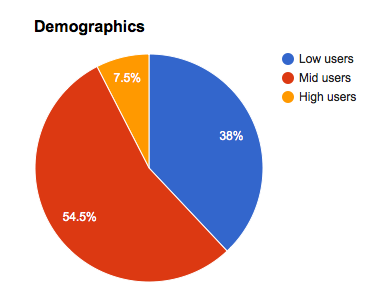
\includegraphics[width=0.5\linewidth]{graphs/demo_split.png}
				\caption{Graph showing the split among the demographics covered in the survey}
				\label{fig:graph-demo-split}
			\end{figure}
			In Appendix A you can find graphical representations of how the respondents to the survey answered each question, these diagrams show the full spectrum of respondents as a whole.\\
			In Appendix B you can find correlation analysis and cross tabulations that we've managed to put together using IBM SPSS Statistics \cite{SPSS}.\\
			We've chosen to include a Sig (2-Tailed) value in our correlation analysis to check if there's a statistically significant correlation between the variables we're measuring. Basically if the value is greater than 0.05 there's no statistically significant correlation else if the value is less or equal to 0.05 there is a statistically significant correlation.\\
			A statistically significant correlation means that a increases or decreases in one of our variables significantly relate to a increases or decreases in our other variable.
			For example, Appendix B Figure B.1 which has a Sig.(2-tailed) value of 0,016 and therefore shows that there's a statistically significant correlation.\\\\
			
			Below you'll see what kind of interfaces the different demographic groups use and below that are graphs displaying what interface our respondents started with and what interface they use today.
			\begin{figure}[H]
					\centering
					\begin{subfigure}[b]{0.315\textwidth}
						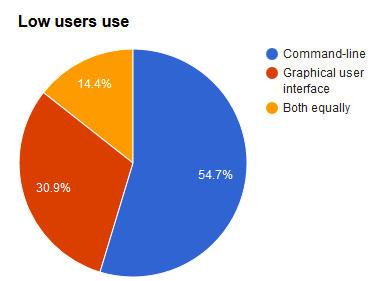
\includegraphics[width=\textwidth]{graphs/low-users-use.png}
						\caption{Low experienced Git users}
						\label{fig:Low users use}
					\end{subfigure}
					~
					\begin{subfigure}[b]{0.315\textwidth}
						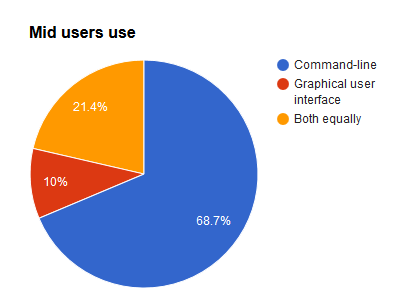
\includegraphics[width=\textwidth]{graphs/mid-users-use.png}
						\caption{Mid experienced Git users}
						\label{fig:Mid users use}
					\end{subfigure}
					~
					\begin{subfigure}[b]{0.315\textwidth}
						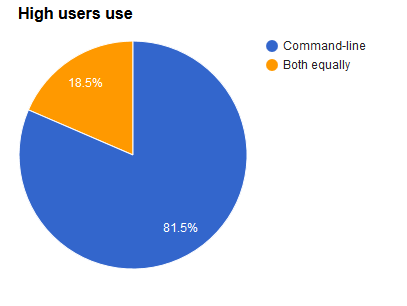
\includegraphics[width=\textwidth]{graphs/high-users-use.png}
						\caption{Highly experienced Git users}
						\label{fig:High users use}
					\end{subfigure}
					\caption{Representation of which interface users indicate that they use depending on demographic}\label{fig:mid-high-users-use}
				\end{figure}
				
				\begin{figure}[H]
					\centering
					\begin{subfigure}[b]{0.45\textwidth}
						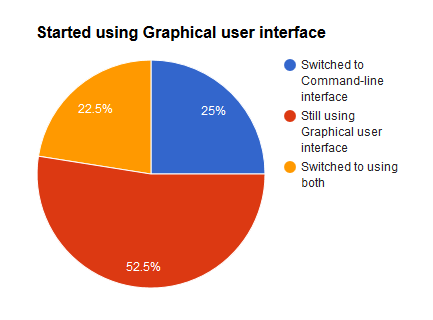
\includegraphics[width=\textwidth]{graphs/started-using-gui.png}
						\caption{Started using GUI - shows what interface respondents use today.}
						\label{fig:started-gui}
					\end{subfigure}
					~
					\begin{subfigure}[b]{0.45\textwidth}
						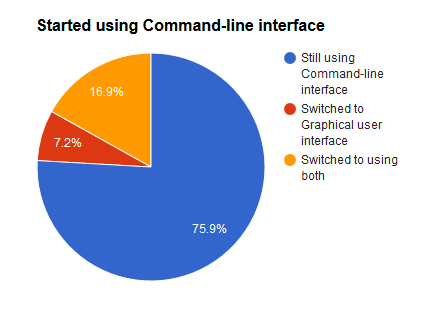
\includegraphics[width=\textwidth]{graphs/started-using-cli.png}
						\caption{Started using CLI - shows what interface respondents use today.}
						\label{fig:started-cli}
					\end{subfigure}
					\caption{Started using - now using.}\label{fig:q9-q10}
				\end{figure}
				
				
				
				
			\section{Interviews}
			The interviews were conducted with three subjects, each interview lasted approximately 5-15 minutes. 
			The more experienced subjects were a little bit more talkative and had more to say on the subject since they have had the time to test other solutions and options, whilst the less experienced subject didn't quite understand all of the questions so we had to try and explain what we meant in an objective way - as best as we could.
			By "in an objective way" - we mean that we avoided positive or negative words that could have influenced the subjects respond.
			A quality analysis has been carried out and the results can be found in Appendix C.
			The full transcripts, in Swedish, of the interviews can be found in Appendix D. The reason of why the transcripts are in Swedish is that the interviews were carried out in Swedish, we felt that a translation could potentially damage the content and therefore we decided not to do it.\\
			
			%\section{User interface analysis}
			%	\begin{center}
			%		\begin{tabular}{ | p{5cm} | c | c | c | }
			%		\hline
			%		Feature & CLI & SourceTree & Smart Git HG \\ 
			%		\hline
			%		Aliases and customizing actions & Yes & Yes & No \\
			%		\hline
			%		Readability of content & Partial & Partial & Yes \\
			%		\hline
			%		Freedom of work flow construction & Yes & Partial & Partial \\
			%		\hline
			%		Ease of setup & Yes & Yes & Yes \\
			%		\hline
			%		Overview ease & Partial & Yes & Yes \\
			%		\hline
			%		Change and branch visualization & Difficult & Partial & Yes \\
			%		\hline
			%		Comprehensive searching & Difficult & Yes & Partial \\
			%		\hline
			%		\end{tabular}
			%		\captionof{table}{UI analysis} \label{tab:UI-Analysis}
			%	\end{center}
			%	\subsection{CLI}
			%	Quite a large amount of functionality in the CLI can be quite advanced, in part giving it a lot of power and flexibility but it becomes more difficult to use. Searching through the change log and files for example can quite easily become complex but the results are very flexible and thus very useful. The same goes for most of the CLI the more specific you want to be and the more demands you have on the interaction the more difficult the process becomes. This is where aliases and custom actions come in handy. They are a way for the user to write the very difficult and complex command once and then call it by an alias of their choosing making the process more affordable.
				%The most notable thing about the CLI is that it lacks very few of the features that the GUIs have, however some of them are very complex to perform in a similar fashion as the GUIs.
			%\subsection{Source Tree}
			%	Source tree has at least partial support for all the features indicating that some of them are either limited or that they are complex to use. It should be mentioned that the UI can become quite cluttered and thus making information confusing to discern, for example viewing the change log along with graphs of the tree structure can be easy to get lost in.
			%	\subsection{Smart Git Hg}
			%	This GUI also had most of the features if not completely then partially. The only thing that was fully missing was the ability to create custom actions and aliases. This UI was more slimmed down than Source Tree and as such got a better score for the Change and branch visualization feature.
		
		% Analysis
		\chapter{Analysis}
				As shown in Appendix A, in Figure A.3(a) the most common interface to get started with - amongst the responders to the survey - is the CLI.
				The majority, 78.2\% percent of the 367 respondents, stated that they started out with Git using the CLI and 21.8\% of the respondents stated that they got started with the GUI.\\
				So to answer RQ1 - CLI is the most common interface used when getting started with Git.
				Diagrams in Figures 5.2b and 5.2c, shows that the command-line dominates amongst the mid to highly experienced users as well. The more experienced the less often they seem to entirely rely on a graphical user interface.\\
				In comparison to 2012's edition of the GitSurvey, 4498 respondents to the question "What Git implementation do you use?" 95\% answered "Git (core) commandline" \cite{GitStructure}.\\	
				The data makes the command-line interface appear to be the most used interface for Git amongst experienced Git users.
				However, it important to note that experience users sometimes use both a command-line interface and a graphical user interface.
				With this in mind, it could be a hint that the users whom use both of the interfaces are missing a feature in the command-line interface that is available in graphical user interfaces.
				Never the less, the answer to RQ2 is the same as for RQ1 - the CLI is most commonly used amongst experienced users as well.\\
				
				Based on the answers we received in our interviews it could very well be that the command-line seem to lack a good visualization of the repository log, something that most graphical user interfaces seem to handle pretty decently.
				A good visualization of the log in the command-line interface is, and we quote, "difficult to do without breaking your fingers" (Bagge, personal communication, May 11, 2015). % Från intervju - Bagge 
				\\\\
				"What can be gained from using the GUI" (RQ3) is a question that is hard to answer, simply because there are a number of different GUI's available and their functionality therefore naturally differs.
				One thing that do appear to be a common phenomenon in graphical user interfaces is the visualisation of the log.
				Another thing that is worth noting is that by using a graphical user interface you do not have to remember all of the commands necessary to commit and push code, for example.\\
				
				Even though the CLI appear to be difficult to new users, see Appendix A Figure A.10, our results claim that it offers more control. The "control"-part seems to be something that all user groups agree on, see Appendix A Figure A.10, A.12 and A.14.
				However, as explained by one of the people we interviewed, a graphical user interface might perform multiple commands when you press one button. This would naturally make it harder to actually understand which commands are executed when a button is pressed (Bjorner, personal communication, May 11, 2015). % Bjorner
				On the contrary, in the CLI you have, unless you've created your own aliases, to type commands manually.
				This leads to us believing that the CLI would provide a better understanding of how Git works in general than a GUI, even though it would require a steeper learning curve.
				Same as for RQ3, RQ4 is tough to answer without a proper UI investigation. But in terms of convenience and when coupled with our data, it would seem that you would gain more control over your workflow in a CLI than a GUI.\\
				%RQ5 START
				\\\\
				Looking at what interface our respondents started out using and what they use today, we can see that out of all the respondents which began using the CLI to interface with Git roughly 76\% of them still use the CLI and only 7.2\% swapped to a graphical user interface, see Figure 5.3(b).
				What it interesting though is that 16.9\% swapped over to use both the CLI and a GUI.
				Meanwhile, if we take a look at the users which began using a graphical user interface about 52\% still use a graphical user interface while 25\% swapped over to the CLI and 22.5\% swapped to both CLI and GUI, see Figure 5.3(a).
				
				There is a strong positive correlation between how experienced the respondents are and how many of them that use the CLI, as seen in Appendix B Figure B.1.
				The same does not apply to the usage of the GUI, because as we can see in Appendix B Figure B.2 there's a strong negative correlation which can be interpreted as the more experience the respondents have the less likely they are to use solely a GUI when interfacing with Git. In fact, none of the highly experienced respondents use a GUI solely (Figure 5.2c).
				\\
				Looking at the cross tabulations we can see that a graphical user interface is more used amongst respondents which learned Git through a friend/colleague or in a course rather than through an open source community, book, online tutorials or by yourself (Appendix B, Figure B.4).\\
				In collaborative work it's more common to use a graphical user interface than working with large scale version control with branch management and code review through Git. About 30\% use a GUI for basic change tracking and collaborative work, whilst only 10\% use it for large scale version control with branch management and code review.\\
				As mentioned earlier, the GUI is used quite often in combination with the CLI, at least when working with large scale version control with branch management and code review.\\
				Another interesting thing, shown in Figure B.6 in Appendix B, is that the type of OS does seem to matter in terms of how many that use the CLI/GUI or both.\\
				In Windows roughly 32\% use a GUI whilst in Mac the number is down to 15,5\% and in Linux 1,5\%.
				From our point of view we believe that those numbers show a correlation between how GUI based a OS is and what type of UI the users use for Git. In that case, it would mean that there's a quite strong negative correlation.
				The same thing could be applied for the GUI whereas roughly 49\% of the Windows users, 61,9\% of the Mac users and 82\% of the Linux users use a CLI which would suggest a strong positive correlation instead.\\\\			
				The correlation analysis put together with the results from the interviews - the fact that the CLI does lack visualization of logs but provide a more controlled environment - shows that graphical user interfaces are more attractive amongst novice users than experienced users.
				But as the users gain experience they seem to swap their GUI for a CLI or to use them both together.\\
				We think it's safe to say that answering RQ5 is close to impossible, if not impossible.
				Our guess is that to answer this question you'd probably have to measure the time it takes to perform typical Git actions in both the GUI and the CLI for a large sample group where the level of experience is very uneven. You would probably have to take in a account that they all work with Git in different ways, someone might just use Git as a way to collaborate with colleagues whilst someone else might use it to review code. Their ways of interacting with Git could be very different. Needless to say, the work required to answer this question would most likely take a tremendous amount of time.
				\\\\
				Our findings summarized in a list:
				\begin{itemize}
					\item The command-line interface is the most widely used interface, amongst all Git users.
					\item The graphical user interface is used less and less by it's own as the user gains experience.
					\item The graphical user interface is still used by highly experienced users but only used together with the CLI and not by its own.
					\item How you learnt Git, what OS you use and what you use Git for - are factors that influence what interface you use. For example, a graphical user interface is much more common amongst Windows users than amongst Mac or Linux users and a graphical user interface is much more common amongst those who learnt Git through a friend/colleague or in a course than amongst those who learnt Git through open source communities or online tutorials.
					\item The general image, provided by the respondents and based on the analyzed data, is that the CLI has a steeper learning curve but offer more control, than the GUI, and the GUI is helpful and simple but contains a lot of auto-magic.
					\item Both interfaces have their pros and cons but it's impossible to say which is the better one, it's all a matter of what you use Git for and your prefered way of working.
					\item According to the interviews we've conducted, graphical user interfaces has detailed logs that are easy to browse through - something that the CLI lacks by default.
					\item The GUI and the CLI has a lot of similarities in terms of functionality, most of the functionality found in the CLI can be found in the GUI such as alias, action customizing and freedom of workflow construction. However, it's hard to say what the exact differences are in terms of convenience and functionality without a proper usability investigation, which is something we didn't have time to do.				 
				\end{itemize}
				
		
		% Conclusion
		\chapter{Conclusion}
		\begin{itemize}
			\item The command-line interface is the most widely used interface, amongst all Git users no matter previous experience.
			\item We have found three major factors that influence what UI is typically used - How you learnt Git, what OS you're using and what you are using Git for in your work.
			\item GUIs are more common amongst novice users and less common amongst experienced users.
			\item It is not unusual that experienced users use a GUI together with a CLI.
			\item It is hard to determine which UI is the better one in terms of functionality and convenience. A proper UI investigation might help in such a regard.
		\end{itemize}
		
		These are the major findings in our work.
		Our guess as to why the CLI is more used than a GUI is that users wants control and it's hard to offer the same type of control in a GUI as the CLI does.
		The entire point of having a GUI is to simplify things, so when you press a button in a GUI you might actually trigger ten different actions in the background - actions that you normally would have to perform one by one in a CLI.\\
		Another thing, that has been mentioned before in the thesis, is that the CLI lacks good visualizations of logs which GUIs seem to do a great job at offering.
		We believe - based on the data we've collected - that this is why a lot of users use both interfaces, a GUI to get good visualizations of logs and the CLI for control.
		
		Three major factors influence what type of interface the users are most likely to use. The first one is how they learnt Git, if they learnt it through a colleague/friend or through a book seems to make a difference. The second factor is what OS they are using, Windows is a more GUI-based OS than Linux. In correlation to that we can see that there is a larger percent of the Git users that use Windows and a GUI for Git than there is Git users that use Linux and a GUI for Git.
		The last factor is what they are using Git for, in collaborative work it is more much common to use a GUI than it is when working with large scale version control with branch management and code review through Git.
		
		It is not uncommon that the GUI is used in combination with the CLI, so it is important to remember that the GUI does play a role for some of the more experienced users.\\
		The use of graphical user interfaces declines as knowledge of Git increases, as shown in the correlation analysis in Appendix B.
		One theory, of ours, of why this is happening is that as a user gains more knowledge he/she will want to optimize his or her workflow to the fullest extent, to save time and to have maximum control. Since roughly 70\% of the respondents associated the CLI with control in comparison to the 11\% that associate the GUI with control it would make sense that the CLI would be significantly favored amongst the experienced Git users.\\
		When speaking of learning, a graphical user interface could be considered a less painful way of learning Git, however you probably don't achieve the same type of control and understanding of Git through a GUI than a command-line interface.
		
		The command-line interface is associated with "control" and "difficult" by the majority of our respondents whilst the GUI is associated with words such as "Simple", "Easy", "Helpful", "Automagic" and "Time consuming".\\
		It is still hard to argue which of the UIs that are the better one, it would probably depend entirely on how you use Git.\\
		
		
		\chapter{Risks}
		There are obvious risks such as people might have filled in the survey more than once. We tried to minimize the risk of that by deleting duplicated entries once all the data was placed in a database based on the respondents email addresses, but since there is an option to not submit the survey with an email address there is a risk that someone might have messed with the results.\\
		Speaking of the interviews on the other hand, the fact that one of our subject didn't have a lot of experience with Git could potentially be a risk as well seeing as we had to explain our questions further at some points which might influence his answer in a way that it shouldn't.
		
		\chapter{Future work}
		It would be interesting to see a complete user interface investigation to see what the actual differences are between the CLI and a GUI. Maybe put a focus on either time consumption when performing certain actions or a focus on customization of actions.\\
		Another thing that would be interesting to find out is if there's any type of milestone, speaking of experience of Git, at which most users swap their interface for another.
		
		% Acknowledgment section
		\chapter*{Acknowledgement}
		We would like to thank our advisor Conny Johansson for his continued support and feedback. The feedback we've received throughout working with this thesis has been very valuable to us.
		
		% References section
		\newpage
		\begin{thebibliography}{1}
			
			\bibitem{GitUserSurvey}
			GitSurvey2012 - Git SCM Wiki. (2012). GitSurvey2012 - Git SCM Wiki. Available: \url{http://git.wiki.kernel.org/index.php/GitSurvey2012}. Last accessed 4th April 2015..
			
			\bibitem{MouseToRat}
			Morgan, K., Morris, R. \& Gibbs, S. (1991). When does a Mouse become a Rat? or … Comparing Performance and Preferences in Direct Manipulation and Command Line Environment. The Computer Journal. 34 (3), p265-271.
			
			\bibitem{MacVsWindows}
			Kirkpatrick, D., Sherman, S., \& Deutschman, A. (1993). Mac vs Windows. Fortune Internc\#ional. 128 (8), p57-64.
			
			\bibitem{GitInClassroom}
			Kelleher, J. (2014, 17-19 Jan). Employing git in the classroom. Paper presented at 2014 World Congress on Computer Applications and Information Systems (WCCAIS). Retrieved 4th April, 2015, at IEEE Xplore. DOI: 10.1109/WCCAIS.2014.6916568.
			
			\bibitem{Treweek}
			Treweek, P. (1996). Comparing Interfaces: Should We Assume that Ease of Use Influences Users' Preference?. Presented at Sixth Australian Conference on Computer-Human Interaction. Retrieved 4th April, 2015, at IEEE Xplore. DOI: 10.1109/OZCHI.1996.560004.
			
			% This is not being used as far as i know.
			%\bibitem{Hart}
			%Hart, D. (2009). A survey of source code management tools for programming courses. Journal of Computing Sciences in Colleges. 24 (6), p113-114.
			
			\bibitem{WrongWithGit}
			Perez De Rosso, S. \& Jackson, D. (2013). What's wrong with git?: a conceptual design analysis. Presented at 2013 ACM international symposium on New ideas, new paradigms, and reflections on programming \& software. Retrieved 4th April, 2015, at ACM Digital Library. DOI: 10.1145/2509578.2509584.
			
			\bibitem{ArtOfUnixProgramming}
			Eric S. Raymond. (2005). The Art of Unix Programming.
			Available: \url{http://www.catb.org/esr/writings/taoup/html/ch11s04.html}.
			Last accessed 6th April 2015.
			
			\bibitem{LinuxGuiVsCli}
			Juergen Haas. Linux: GUI vs. Command line. Available: \url{http://linux.about.com/cs/softofficeutility/a/gui\_cli.htm}. Last accessed 6th April 2015.
			
			\bibitem{GithubAbout}
			Github.com - Features. (2015). Available: \url{https://github.com/features/}. Last accessed 16th April 2015.
			
			\bibitem{ProGit}
			S. Chacon, Pro Git, New York, NY: Apress, 2009.
			
			\bibitem{EclipseDeveoperReport}
			The Eclipse Foundation. "Eclipse Open Source Developer Report". The Eclipse Foundation. San Francisco, CA. 2012.
			
			\bibitem{DeveloperProductivity}
			ZeroTurnaround. "Developer Productivity Report 2012: Java Tools, Tech, Devs \& Data". ZeroTurnaround. Boston, MA. 2012.
			
			\bibitem{MicrosoftSurveyResults}
			Microsoft Corporation, "Survey Results: Open Source Developer Preferences (June 2011)," Microsoft Corporation, 11 July 2011. [Online]. Available: \url{http://blogs.msdn.com/b/codeplex/archive/2011/07/11/survey-results-open-source-developer-preferences-june-2011.aspx}. [Accessed 18th April 2015].
			
			\bibitem{WhatIsGui}
			Webopedia.com. (2015). Available: \url{http://www.webopedia.com/TERM/G/Graphical\_User\_Interface\_GUI.html}. [Accessed 18th April 2015].
			
			\bibitem{FoundationVCforWebDevs}
			C. Kemper and I. Oxley. Foundation Version Control for Web Developers. Berkeley, CA: Apress. 2012.
			
			\bibitem{HistoryOfGUIWiki}
			Wikipedia. (Unknown). History of the graphical user interface. Available: \url{http://en.wikipedia.org/wiki/History_of_the_graphical_user_interface#Apple_Lisa_and_Macintosh_.28and_later.2C_the_Apple_IIgs.29}.  [Accessed 20th April 2015].
			
			\bibitem{lootcrate}
			Loot Crate. Available: \url{www.lootcrate.com} [Accessed 20th April 2015]
			
			\bibitem{GoogleSpreadsheet}
			Google Spreadsheet. Available: \url{https://www.google.se/intx/sv/work/apps/business/products/sheets/?utm_source=google&utm_medium=cpc&utm_campaign=emea-se-sv-drive-bkws-all-trial-e&utm_term=google%2Bkalkylark} [Accessed 26th April 2015]
			
			\bibitem{GitStructure}
			Unlearn what you have learned. (2014). Git: How it works. Available: \url{http://bartoz.no-ip.org/archives/2981}. [Accessed 14th May 2015].
			
			\bibitem{GitGUIs}
			Git SCM. GUI Clients. Available: \url{http://git-scm.com/downloads/guis}. [Accessed 14th May 2015].
			
			\bibitem{InTheBeginning}
			Neal Stephenson. (1999). In the Beginning was the Command Line. Available: \url{http://cristal.inria.fr/~weis/info/commandline.html}	[Accessed: 14th May 2015].
			
			\bibitem{vcsExplanation}
			Spinellis, D. 2005. Version control systems. IEEE Software 22, (5): 108-109	
			
			\bibitem{typesOfVCS}
			Git SCM. Getting Started - About Version Control. Available: \url{https://git-scm.com/book/en/v2/Getting-Started-About-Version-Control}. [Accessed 3rd August 2015].
			
			\bibitem{OracleCLIAndGUI}
			Chapter 1 Differences Between Command Line Interface and Graphical User Interface (Solaris Advanced User's Guide). Available: \url{http://docs.oracle.com/cd/E19683-01/806-7612/startup-78447/index.html} [Accessed 10th August 2015].
			
			\bibitem{SPSS}
			IBM SPSS Statistics. Available: \url{http://www-01.ibm.com/software/analytics/spss/products/statistics/} [Accessed 10th August 2015].
			\bibitem{WhyGit}
			Giancarlo Lionetti. (2012). Git vs Mercurial: Why Git?.
			Available: \url{http://blogs.atlassian.com/2012/03/git-vs-mercurial-why-git/}.
			Last accessed 6th September 2015.
			
		\end{thebibliography}
		
		\appendix
		\chapter{Data from survey}
		\begin{figure}[H]
			\centering
			\begin{subfigure}[b]{0.45\textwidth}
				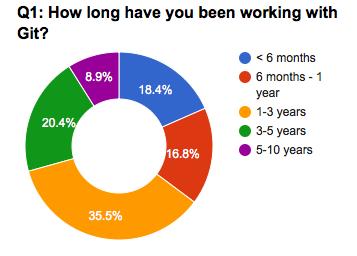
\includegraphics[width=\textwidth]{graphs/q1.png}
				\caption{Representation of results of question 1}
				\label{fig:q1}
			\end{subfigure}
			~
			\begin{subfigure}[b]{0.45\textwidth}
				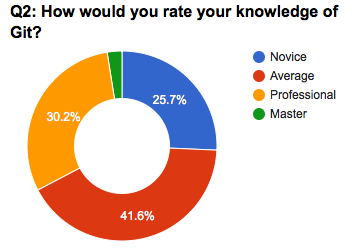
\includegraphics[width=\textwidth]{graphs/q2.png}
				\caption{Representation of results of question 2}
				\label{fig:q2}
			\end{subfigure}
			\caption{Questions 1 and 2}\label{fig:q1-q2}
		\end{figure}
		\begin{figure}[H]
			\centering
			\begin{subfigure}[b]{0.45\textwidth}
				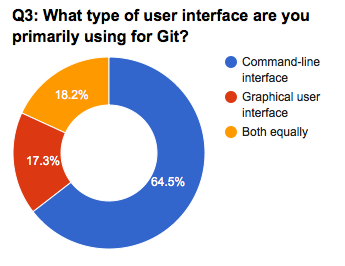
\includegraphics[width=\textwidth]{graphs/q3.png}
				\caption{Representation of results of question 3}
				\label{fig:q3}
			\end{subfigure}
			~
			\begin{subfigure}[b]{0.45\textwidth}
				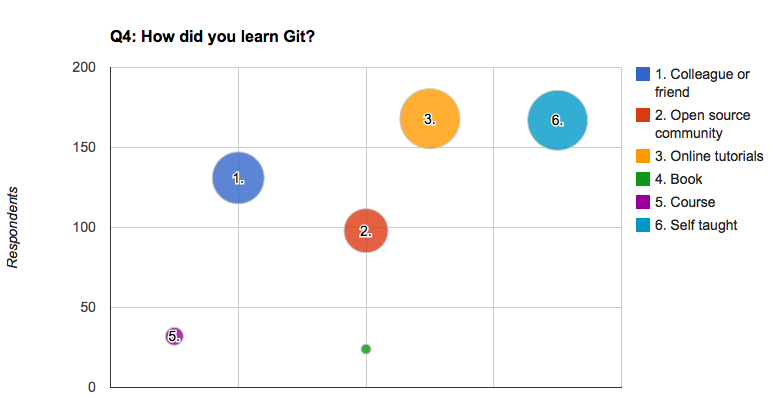
\includegraphics[width=\textwidth]{graphs/q4.png}
				\caption{Representation of results of question 4}
				\label{fig:q4}
			\end{subfigure}
			\caption{Questions 3 and 4}\label{fig:q3-q4}
		\end{figure}
		\begin{figure}[H]
			\centering
			\begin{subfigure}[b]{0.45\textwidth}
				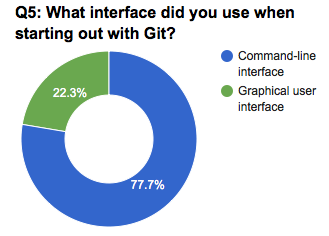
\includegraphics[width=\textwidth]{graphs/q5.png}
				\caption{Representation of results of question 5}
				\label{fig:q5}
			\end{subfigure}
			~
			\begin{subfigure}[b]{0.45\textwidth}
				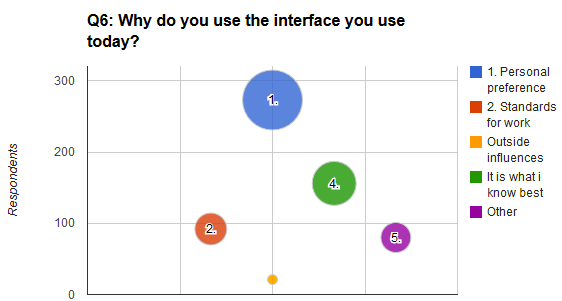
\includegraphics[width=\textwidth]{graphs/q6.png}
				\caption{Representation of results of question 6}
				\label{fig:q6}
			\end{subfigure}
			\caption{Questions 5 and 6}\label{fig:q5-q6}
		\end{figure}
		\begin{figure}[H]
			\centering
			\begin{subfigure}[b]{0.45\textwidth}
				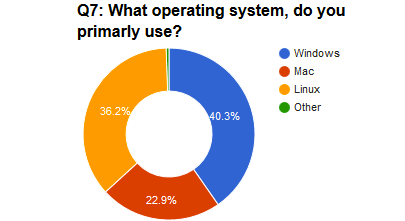
\includegraphics[width=\textwidth]{graphs/q7.png}
				\caption{Representation of results of question 7}
				\label{fig:q7}
			\end{subfigure}
			~
			\begin{subfigure}[b]{0.45\textwidth}
				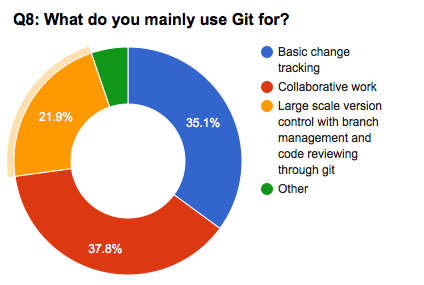
\includegraphics[width=\textwidth]{graphs/q8.png}
				\caption{Representation of results of question 8}
				\label{fig:q8}
			\end{subfigure}
			\caption{Questions 7 and 8}\label{fig:q7-q8}
		\end{figure}
		\begin{figure}[H]
			\centering
			\begin{subfigure}[b]{0.45\textwidth}
				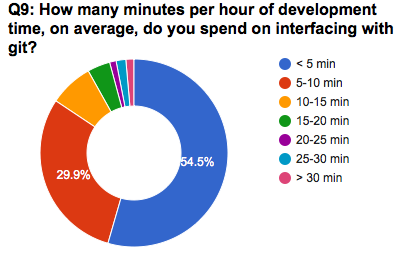
\includegraphics[width=\textwidth]{graphs/q9.png}
				\caption{Representation of results of question 9}
				\label{fig:q9}
			\end{subfigure}
			~
			\begin{subfigure}[b]{0.45\textwidth}
				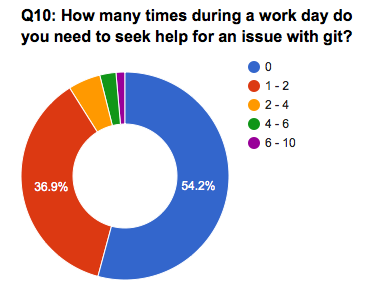
\includegraphics[width=\textwidth]{graphs/q10.png}
				\caption{Representation of results of question 10}
				\label{fig:q10}
			\end{subfigure}
			\caption{Questions 9 and 10}\label{fig:q9-q10}
		\end{figure}
		\begin{figure}[H]
			\centering
			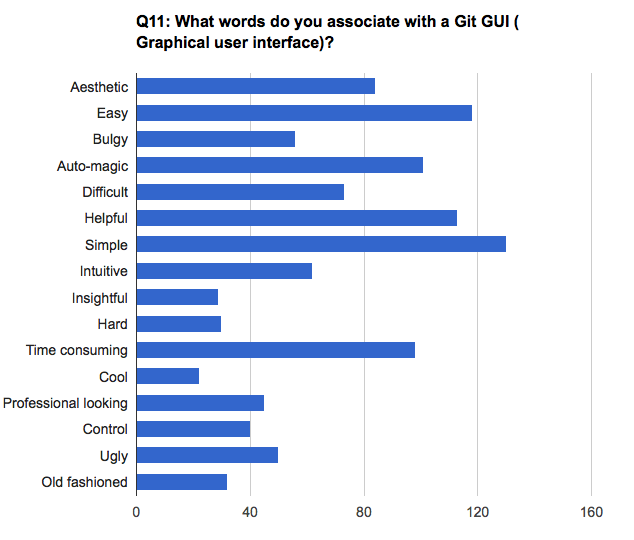
\includegraphics[width=0.8\linewidth]{graphs/q11.png}
			\caption{Representation of results of question 11}
			\label{fig:q11}
		\end{figure}
		\begin{figure}[H]
			\centering
			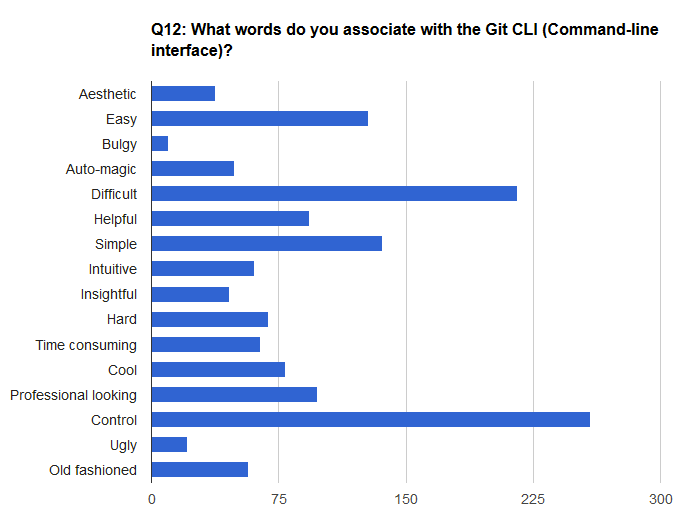
\includegraphics[width=0.8\linewidth]{graphs/q12.png}
			\caption{Representation of results of question 12}
			\label{fig:q12}
		\end{figure}
		\begin{figure}[H]
			\centering
			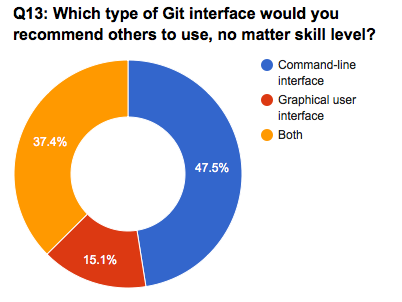
\includegraphics[width=0.5\linewidth]{graphs/q13.png}
			\caption{Representation of results of question 13}
			\label{fig:q13}
		\end{figure}
		
		\begin{figure}[H]
			\centering
			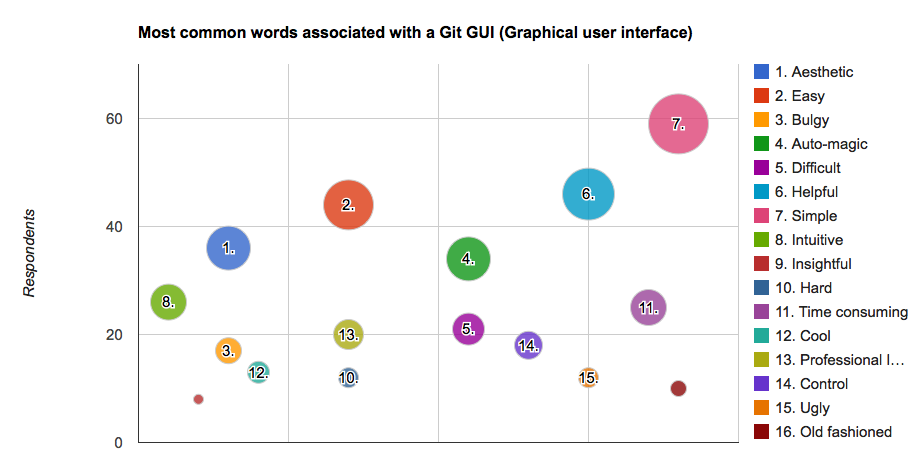
\includegraphics[width=0.95\textwidth]{graphs/common-words-low-users-gui.png}
			\caption{Low experienced Git users - common words associated with Git GUI.}
			\label{fig:Low users - common words associated with Git GUI.}
		\end{figure}
		\begin{figure}[H]
			\centering
			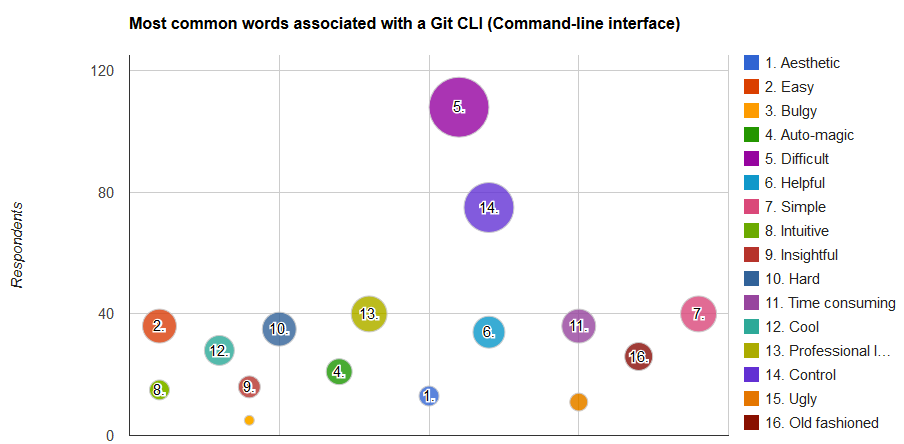
\includegraphics[width=0.95\textwidth]{graphs/common-words-low-users-cli.png}
			\caption{Low experienced Git users - common words associated with Git CLI.}
			\label{fig:Low users - common words associated with Git CLI.}
		\end{figure}
		\begin{figure}[H]
			\centering
			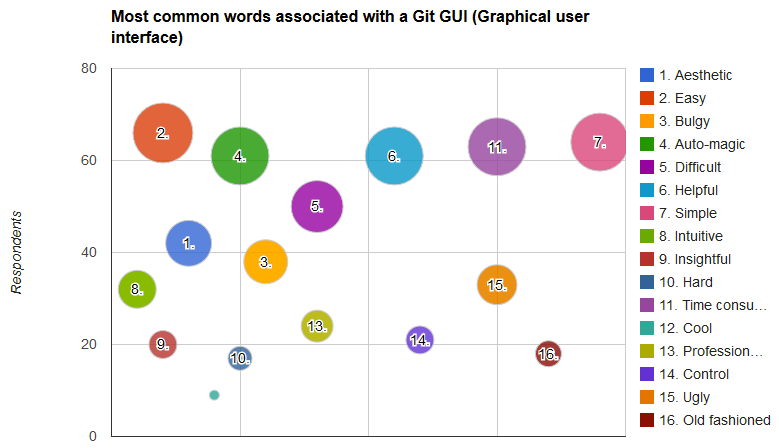
\includegraphics[width=0.95\textwidth]{graphs/common-words-mid-users-gui.png}
			\caption{Mid experienced Git users - common words associated with Git GUI.}
			\label{fig:Mid users - common words associated with Git GUI.}
		\end{figure}
		\begin{figure}[H]
			\centering
			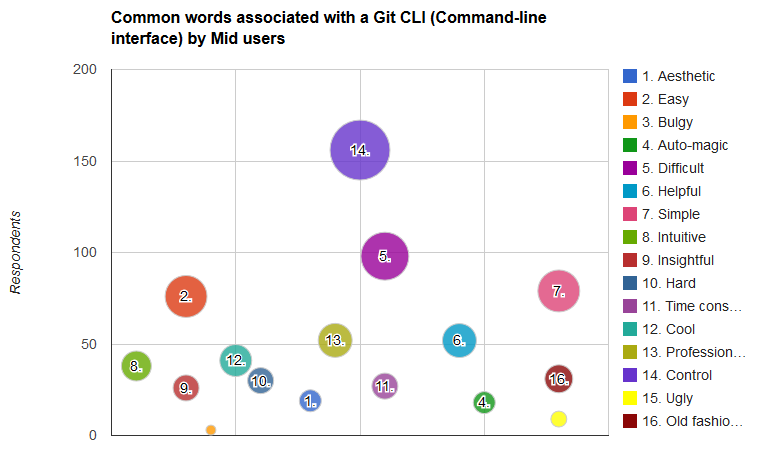
\includegraphics[width=0.95\textwidth]{graphs/common-words-mid-users-cli.png}
			\caption{Mid experienced Git users - common words associated with Git CLI.}
			\label{fig:Mid users - common words associated with Git CLI.}
		\end{figure}
		\begin{figure}[H]
			\centering
			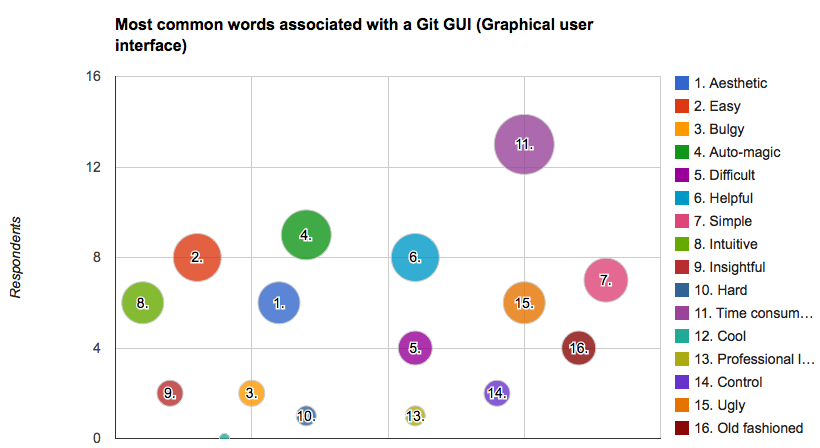
\includegraphics[width=0.95\textwidth]{graphs/common-words-high-users-gui.png}
			\caption{Highly experienced Git users - common words associated with Git GUI.}
			\label{fig:High users - common words associated with Git GUI.}
		\end{figure}
		\begin{figure}[H]
			\centering
			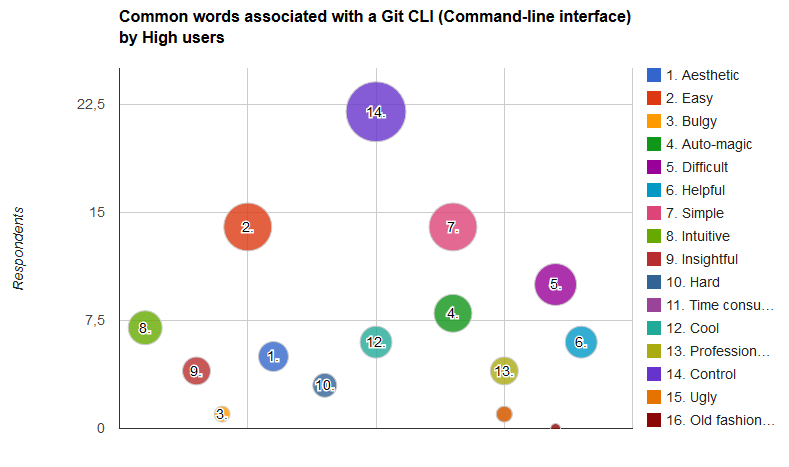
\includegraphics[width=0.95\textwidth]{graphs/common-words-high-users-cli.png}
			\caption{Highly experienced Git users - common words associated with Git CLI.}
			\label{fig:High users - common words associated with Git CLI.}
		\end{figure}	
		
		\chapter{Correlation Analysis \& Cross tabulations}
		\begin{figure}[H]
			\centering
			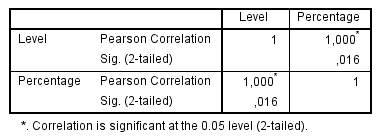
\includegraphics[width=0.75\textwidth]{graphs/correlation-between-knowledge-and-usage-of-cli.png}
			\caption{Correlation between experience and usage of the CLI. Shows that as experience (in the analysis referred to level) increase the number of CLI users increase. Sig-value of 0.016 which shows a statistically significant correlation.}
			\label{fig:Correlation between experience and usage of the CLI.}
		\end{figure}
		
		\begin{figure}[H]
			\centering
			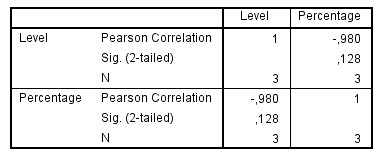
\includegraphics[width=0.75\textwidth]{graphs/correlation-between-knowledge-and-usage-of-gui.png}
			\caption{Correlation between experience and usage of the GUI. Shows that as experience (in the analysis referred to as level) increases the number of GUI users decreases. Sig-value of 0.128 which shows that there is no statistically significant correlation.}
			\label{fig:Correlation between experience and usage of the GUI.}
		\end{figure}
		
		\begin{figure}[H]
			\centering
			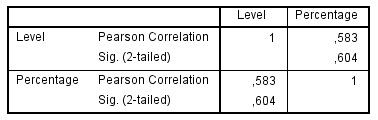
\includegraphics[width=0.75\textwidth]{graphs/correlation-between-knowledge-and-usage-of-both.png}
			\caption{Correlation between experience and usage of both the CLI and GUI. Shows that as experience (in the analysis referred to as level) increases the number of users, that use both a GUI and the CLI, increases. Sig-value of 0.128 which shows that there is no statistically significant correlation.}
			\label{fig:Correlation between experience and usage of both the CLI and GUI.}
		\end{figure}
		
		\begin{figure}[H]
			\centering
			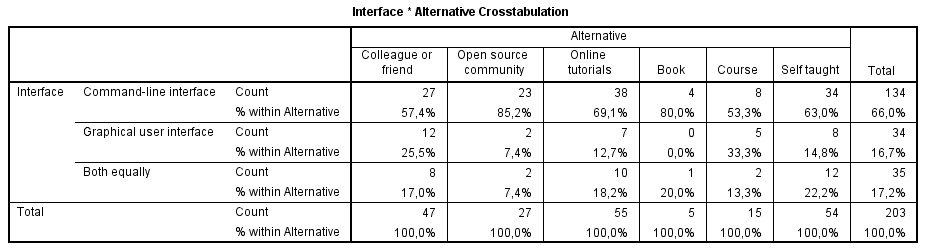
\includegraphics[width=1\textwidth]{graphs/crosstabulation-learnt-using.png}
			\caption{A cross tabulation showing how many that learnt Git through each of the options available in question 4, in the survey, and what interface they are using now.}
			\label{fig:cross tabulation - what interface they are using x how they learnt Git}
		\end{figure}
		
		\begin{figure}[H]
			\centering
			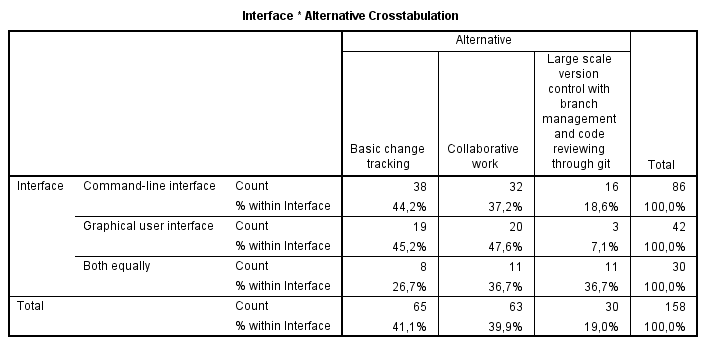
\includegraphics[width=1\textwidth]{graphs/crosstabulation-how-using-git-interface.png}
			\caption{A cross tabulation showing what respondents use Git for and what interface they are using for their work.}
			\label{fig:cross tabulation - what interface they are using x what they use Git for.}
		\end{figure}
		
		\begin{figure}[H]
			\centering
			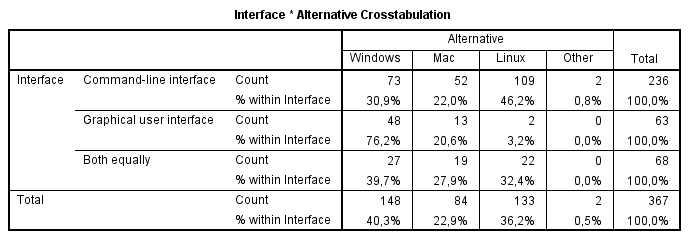
\includegraphics[width=1\textwidth]{graphs/crosstabulation-os-using.png}
			\caption{A cross tabulation showing what OS respondents use and what interface they are using.}
			\label{fig:cross tabulation - what interface they are using x what OS they use.}
		\end{figure}
		
		\chapter{Quality Analysis of interviews}
		\subsection{Bagge}
		The command that the respondent uses the most is git grep, a command that the respondent is unsure about if it exists in a GUI.
		
		The respondent has used graphical user interfaces in the past, but it would appear as if it doesn’t occur that often. But he knows about tortoiseGit and GitK, he also talks a little bit about tig. So it’s safe to say that he has some knowledge about what’s out there in terms of GUIs.
		
		The respondent also explains why he’s not working in a GUI environment by talking about the fact that he doesn’t have a workflow for it so he doesn’t really know what to do.
		
		When talking about tig, he mentions that the CLI lacks a visualization of the log. He also mentions that you could create your own visualization of the log in a CLI but that it’s hard to do.
		
		When asked how he feels about working using the CLI in comparison to a GUI, he says that the CLI feels like home. It is in the CLI where he does his works.
		
		
		\subsection{Bjorner}
		The respondent mainly uses Git for branch managing and has used a GUI quite often in the past. He thinks that the GUI is great for log visualizations, he thinks that he can easily get a good overview of the repository history. He uses the CLI as his primary interface.
		
		The respondent believes that the GUI is a good starting point for new Git users that aren’t used to working in a CLI.
		
		He, himself, is very comfortable working in the CLI because it provides a feeling of control.
		
		The respondent doesn’t think that he gains anything by using a GUI when working alone but feels that it’s useful when working together with someone else when - for example - browsing through repository history.
		
		
		\subsection{Eliasson}
		The main functionality the respondent uses is the git clone command, to clone repositories.
		He does not have much experience with working with GUIs, he primarily uses a CLI.
		
		The respondent does not have much experience working with a CLI either, but feels like it’s hard to tell when something goes wrong when using a CLI.
		He says that; going from a GUI to a CLI is a little bit wierd, you don’t always keep track of where you are (assumingly where you are in terms of Git events, directories etc.).
		So one thing he misses from the GUI is some kind of indication of where he is and what he’s doing in the CLI.
		
		\chapter{Transcripts of the interviews}
		\subsection{Bagge}
		\textbf{sebastian:} Vilken funktionalitet använder du oftast? eller vilka funktionaliteter är det du vanligtvis använder?
		\\\textbf{respondent:} Gissningsvis är det kommandot som jag mest använder git grep.
		\\\textbf{sebastian:} Git grep?
		\\\textbf{respondent:} Ja, för att leta i källkoden liksom efter någonting.
		\\\textbf{sebastian:} Men det git grep är ingenting som egentligen finns tillgängligt i grafiska gränssnitt, va?
		\\\textbf{respondent:} Oj, det har jag ingen aning om.
		\\\textbf{respondent:} Det hade ju varit rätt praktiskt om jag öppnade min källkod i en sån källkodsbrowser-grej, för det blir det ju i det fallet, så skulle jag ju kunna tänka mig göra grep i den liksom.
		\\\textbf{sebastian:} Hur upplever du att det är att arbeta med ett grafiskt interface emot Git? Jag gissar att du har gjort det någon gång åtminstone.
		\\\textbf{respondent:} Ja, det händer ju. Det beror ju lite på vad man lägger det emot förstås. Men om man tar dem strikt grafiska typ tortoiseGit och GitK och…
		\\\textbf{sebastian:} SourceTree?
		\\\textbf{respondent:} Det har jag aldrig hört talas om, eller har hört talas om det men aldrig använt det. Det är väll egentligen tortoiseGit och GitK som jag använt.
		Sen har man dem som är borderline typ tig, som är ganska så trevligt när man gör vissa grejer.
		Jag kan egentligen inte arbeta i dom (grafiskt interface mot Git), är väll det rent praktiska i det.
		\\\textbf{sebastian:} Okej, på vilket sätt?
		\\\textbf{respondent:} Jag har inget arbetsflöde för det så jag vet inte hur jag ska göra. Så jag har använt det någon gång då och då för att titta på olika saker av olika skäl.
		Det är inget för mig.
		Tig har jag använt för att den har någon visualisering av loggen som är helt underbar liksom.
		Men det va längesen jag använde det senast. Så på något vis har jag väll inte behövt det, det är väll typ när man ska ner i loggen och leta långt bak och så ska man försöka förstå hur det hänger ihop så har den ett litet läge för att visa loggen med olika bakgrunder med histogram och sånt. Så att den har en funktion där som saknas lite på kommandoraden, eller den är svår att göra på kommandoraden utan att knäcka fingrarna.
		\\\textbf{sebastian:} Nästa fråga då, ur upplever du att det är att arbeta med ett CLI emot Git?
		\\\textbf{respondent:} Det är där jag bor liksom, jag jobbar med kommandoradsprylar. I det som jag producerar på jobbet så är det ju kommandoradsprylar. Att då jobba i kommanrodaden känns då som.. det vore lite löjligt att sitta och skriva kommandoradsprogram och sen jobba på ett annat sätt.
		Eftersom jag ändå sitter i en terminal när jag ändå ska prova koden så varför ska jag inte göra Git kommandon där i samma terminal. Någonstans där finns det en connection. 
		Sen förövrigt så finns det ett flöde där som jag har vant mig vid.
		\\\textbf{sebastian:} Vad saknar du ifrån ett GUI som du skulle vilja ha möjlighet att använda i ett CLI?
		\\\textbf{respondent:} Det finns ju en grej som jag saknar när det kommer till loggen som jag egentligen inte tycker finns i någon utav dem som jag har provat.
		Det är att om jag vill titta på loggen så vill jag smidigt kunna följa ändringarna och sånt och det är komplicerat. Det är ju egentligen för att Git är byggt så som det är med förändringarna och sånt, så det är nog komplicerat att skriva ett kompetent UI oavsett vilken väg man väljer.
		Om du har den här ändringen kan du visa allt som har med den att göra med en snygg kedja som blir logisk för människohjärnan, för tyvärr är det ju så att göra det datalogiskt med hur dom hänger ihop är ju inte så komplicerat men det är inte så dom hänger ihop för mig som människa när jag tittar på ändringarna. Så ändringar kan komma fel, rent strukturellt, i mitt huvud jämfört med hur dom händer i trädet.
		Det finns en önskan om att loggen kanske kunde varit lite mer tillgänglig.
		\\\textbf{sebastian:} Finns det någon tidsaspekt som du skulle kunna optimera om du hade ett grafiskt gränssnitt istället för ett CLI?
		\\\textbf{respondent:} svaret är nej, för min del. Jag sitter aktivt och skriver raderna, men jag är ganska snabb på det för att jag vet vilken ordning allt ska vara i.
		\\\textbf{sebastian:} Ja, det är väll muskelminne vid det här laget.
		\\\textbf{respondent:} Ja.
		\\\textbf{sebastian:} Som summering på sista frågan så kan man säga att du har en del alias, du har tre totalt.
		\\\textbf{respondent:} Ja, det är dom som jag använder iallafall.
		\\\textbf{sebastian:} Som gör dig lite smidigare, även om ett utav dom åtminstone är inte att rekommendera. Det är det du tycker gör saker och ting lättare och du saknar ingenting annat ifrån Guit.
		\\\textbf{respondent:} Nej, inte medvetet iallafall.
		\\\textbf{sebastian:} Förutom just då Tig-grejerna.
		\\\textbf{respondent:} Ja, på sätt och vis så skulle det kunna vara så att jag har ju inte använt det så jag vet ju inte.
		
		
		
		
		\subsection{Bjorner}
		\textbf{sebastian:} Vilken funktionalitet i Git anser du att du jobbar med oftast, eller vilka funktionaliteter arbetar du mest med?
		\\\textbf{respondent:} Jag skulle väll säga att jag för det mesta arbetar, just inom Git, med branchning för att lätt kunna experimentera loss i projekt jag sitter i utan att behöva ta sönder någonting i master.
		Jag använder det för att kunna ha en egen kopia utav våran källkod på jobbet, som jag arbetar med, utan att jag stör någon annan. Att, ja, implementera.
		\\\textbf{sebastian:} Så branchmanagement i Git är det du pysslar med mest?
		\\\textbf{respondent:} Ja, om man ändå bortser från det vanliga med commits.
		\\\textbf{sebastian:} Hur upplever du att arbeta med ett GUI? Hur ser du på arbetet med det?
		\\\textbf{respondent:} Jag har själv kört en del GUIn till Git. Inte så mycket GitGTK som är det vanliga, som man får med Git utan jag har använt SoureTree som är skapat av Atlassian.
		Jag tycker att GUIn är väldigt bra för att notera data, så du får snabbt en bra överblick över hur t.ex. hur ser din historik i Git. Du får data presenterat på ett väldigt vänligt sätt i GUIt, tycker jag överlag.
		\\\textbf{sebastian:} Är det någonting mer du vill tillägga på GUI delen?
		\\\textbf{respondent:} Ja, asså om man ska kolla på det hela så även med lite mer avancerade verktyg som har en terminalsida till det så tror jag att GUIn är en väldigt bra inkörningsport om man inte är så bekväm vid att sitta i en terminal.
		\\\textbf{sebastian:} Samma fråga, fast riktat mot CLI.
		\\\textbf{respondent:} Ja, jag trivs väldigt bra i terminalen för det känns som att jag har mycket mer kontroll över vad som händer i och med att verktygen ofta automatiserar långa kedjor utav kommandon baserat på vart du trycker. Om du trycker på en knapp så kan det vara fem eller sex kommandon som exekveras i ett GUI medans här får man göra allting verkligen för hand.
		Det kan ta mycket längre tid, det kan ta kortare tid beroende på hur van man är. Men jag känner att jag har mer kontroll i terminalen.
		\\\textbf{sebastian:} Vad saknar du, om något, i det gränssnitt som du använder idag? Jag gissar på att det är CLI du använder idag?
		\\\textbf{respondent:} Jajamen, det är det. Det jag saknar är väll lite som jag pratade om när jag pratade GUI, att snabbt kunna få en bra visuell representation utav saker. Jag kan inte, ur ren standard, få en bra representation utav min historik utan att kunna massa specialkommandon i Git tillexempel.
		\\\textbf{sebastian:} Så dem grafiska egenskaperna är något som du känner gör arbetet med det mer lättar att hantera och lite effektivare?
		\\\textbf{respondent:} Det beror helt på, om jag sitter själv och jobbar så tycker jag inte riktigt att det riktigt tjänar mig någonting att ha något grafiskt.
		Men om man ska sitta tillsammans med någon och kanske förklara någonting eller gå igenom en historik, då känner jag att det är mycket lättare att ha ett grafiskt gränssnitt att arbeta igenom.
		
		
		
		\subsection{Eliasson}
		\textbf{Sebastian:} Vilken funktionalitet i Git är det du använder oftast, vilken eller vilka?
		\\\textbf{Respondent:} Det är mestadels för att klona grejer som andra har gjort.
		\\\textbf{Sebastian:} Så bara hämta källkod för att kolla på?
		\\\textbf{Respondent:} Ja.
		\\\textbf{Sebastian:} Hur upplever du att det är att arbeta med Guit eller någon utav Guina som finns tillgänliga för Git?
		\\\textbf{Respondent:} Jag har ju inte jobbat mycket alls med Guit, men det har ju varit bra hittills.
		\\\textbf{Sebastian:} Är det någonting du tycker är extra trevligt i Guina eller extra kasst i Guina, som du har märkt.
		\\\textbf{Respondent:} Nej, jag kan nog inte säga det.
		\\\textbf{Sebastian:} Då går vi vidare till samma fråga fast för kommandoraden.
		\\\textbf{Respondent:} Det har funkat bra, i och med att jag inte har använt det så mycket så har jag svårt att säga vad som är problematiskt. Man måste sitta lite med grejer för att märka av att det inte riktigt funkar som jag vill. Det är svårt att utmärka problem.
		\\\textbf{Sebastian:} Det är ju problem ifrån din synvinkel, det ska inte vara buggar i systemet. Utan hur du uppfattar det.
		\\\textbf{Respondent:} Nej, det förstår jag. Men jag har inte använt det tillräckligt mycket, känner jag.
		\\\textbf{Sebastian:} Är det någonting du tycker är extra svårt, som typ branchhantering eller commithantering eller rebase?
		\\\textbf{Respondent:} Det jag känner framför allt är att jag är ovan att skriva det på det sättet, men hittills har det funkat bra.
		\\\textbf{Sebastian:} Hur mycket erfarenhet har du haft av kommandoraden tidigare innan du började använda Git?
		\\\textbf{Respondent:} Jag läste ju Linux på gymnasiet.
		\\\textbf{Sebastian:} De var en kurs eller?
		\\\textbf{Respondent:} Det var en kurs, jag läste den cirka en termin. Om jag inte kommer ihåg helt fel så var jag rätt intresserad tillochmed. Men man tappar det snabbt, tyvärr.
		\\\textbf{Sebastian:} Jo, så blir det tyvärr. När man inte jobbar med det mycket så försvinner det ganska fort. Men det är det rättvist att säga att du inte är jättevan vid att använda terminaler och sånt?
		\\\textbf{Respondent:} Det börjar komma tillbaka, men jag är fortfarande ovan.
		\\\textbf{Sebastian:} Vad saknar du, om något, i gränssnittet som du använder idag? Alltså vad saknar du i CLI:t för att bli mer effektiv, för att vara smidigare att använda, för att göra saker och ting lättare för dig i utveckling och arbetet med Git?
		\\\textbf{Respondent:} Från ett GUI till en kommandorad blir lite sådär små konstigt, man håller inte hela tiden koll på vart man är och så. Det är framför allt det jag känner att jag saknar, att jag vill ha någonting som indikerar vart jag är någonstans hela tiden.
		\\\textbf{Sebastian:} Ja, precis. För man tappar bort sig litegranna ibland.
		\\\textbf{Respondent:} Ja.
		\\\textbf{Sebastian:} Jag gissar på att du inte har hållit på någonting med changeloggar och grafer och såntdär än?
		\\\textbf{Respondent:} Nej.
		

\end{document}
